\documentclass[tikz,border=5pt]{standalone}
\usepackage{fontspec,amsmath,amssymb}
\IfFontExistsTF{Times New Roman}{\setmainfont{Times New Roman}}{\setmainfont{Latin Modern Roman}}
\IfFontExistsTF{Arial}{\setsansfont{Arial}}{\setsansfont{Latin Modern Sans}}
\usetikzlibrary{arrows.meta,positioning,calc}
\definecolor{ink}{HTML}{20364A}
\definecolor{bluewash}{HTML}{EDF3F7}
\definecolor{greenwash}{HTML}{EFF5F1}
\tikzset{box/.style={draw=ink!65,fill=white,line width=.5pt,rounded corners=1.5pt,align=left,inner sep=5pt,font=\sffamily\fontsize{8}{10}\selectfont},arr/.style={-{Stealth[length=2mm]},draw=ink,line width=.7pt},head/.style={font=\sffamily\bfseries\fontsize{10}{12}\selectfont,text=ink,anchor=west},note/.style={font=\sffamily\fontsize{7.5}{9}\selectfont,text=ink,align=left}}
\begin{document}
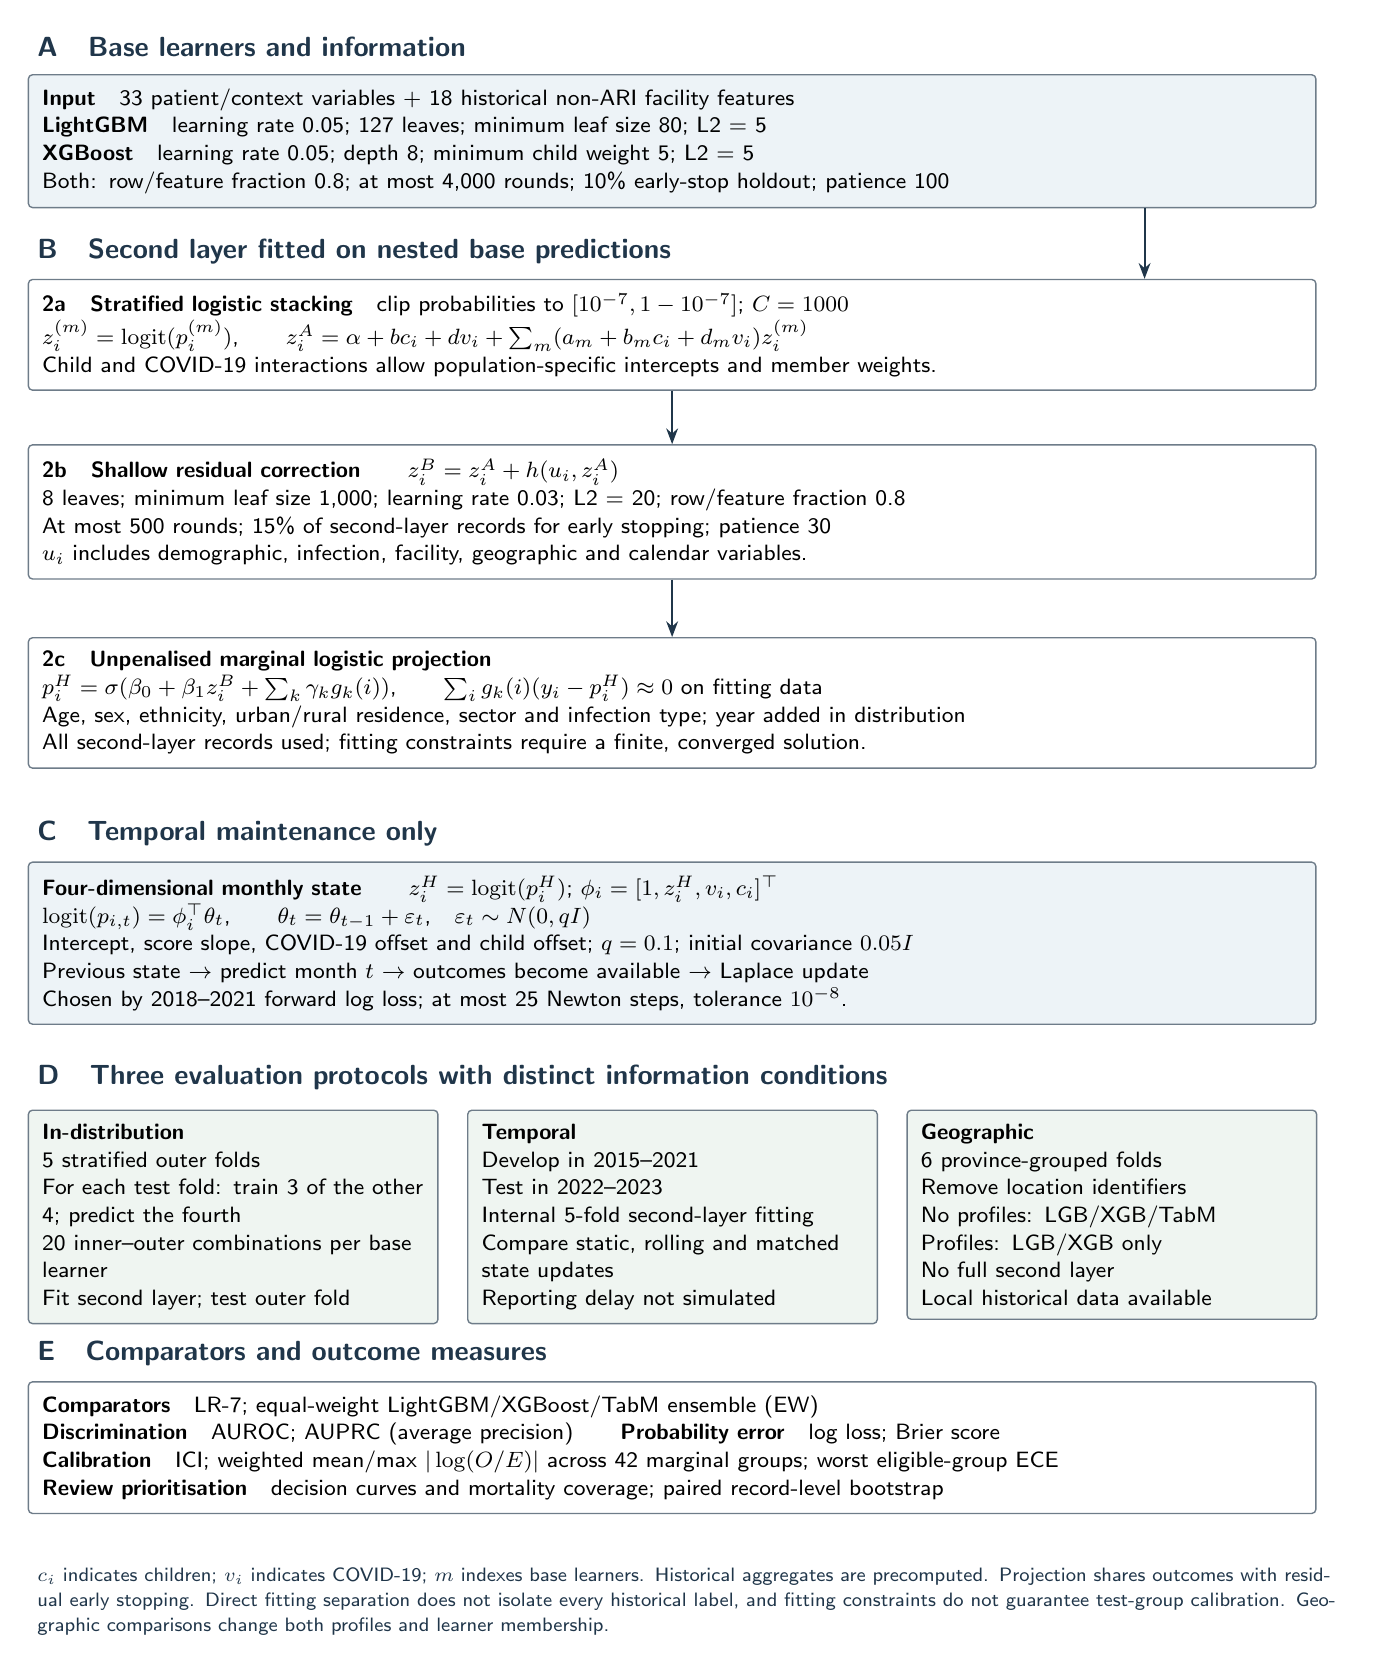
\begin{tikzpicture}[x=1cm,y=1cm]

\node[head] at (0,0) {A\quad Base learners and information};
\node[box,fill=bluewash,text width=16cm,anchor=north west] (input) at (0,-.35) {\textbf{Input}\quad 33 patient/context variables + 18 historical non-ARI facility features\\\textbf{LightGBM}\quad learning rate 0.05; 127 leaves; minimum leaf size 80; L2 = 5\\\textbf{XGBoost}\quad learning rate 0.05; depth 8; minimum child weight 5; L2 = 5\\Both: row/feature fraction 0.8; at most 4,000 rounds; 10\% early-stop holdout; patience 100};
\node[head] at (0,-2.6) {B\quad Second layer fitted on nested base predictions};
\node[box,text width=16cm,anchor=north west] (stack) at (0,-2.95) {\textbf{2a\quad Stratified logistic stacking}\quad clip probabilities to $[10^{-7},1-10^{-7}]$; $C=1000$\\$z_i^{(m)}=\operatorname{logit}(p_i^{(m)})$,\qquad $z_i^A=\alpha+bc_i+dv_i+\sum_m(a_m+b_mc_i+d_mv_i)z_i^{(m)}$\\Child and COVID-19 interactions allow population-specific intercepts and member weights.};
\node[box,text width=16cm,anchor=north west] (resid) at (0,-5.05) {\textbf{2b\quad Shallow residual correction}\qquad $z_i^B=z_i^A+h(u_i,z_i^A)$\\8 leaves; minimum leaf size 1,000; learning rate 0.03; L2 = 20; row/feature fraction 0.8\\At most 500 rounds; 15\% of second-layer records for early stopping; patience 30\\$u_i$ includes demographic, infection, facility, geographic and calendar variables.};
\node[box,text width=16cm,anchor=north west] (proj) at (0,-7.5) {\textbf{2c\quad Unpenalised marginal logistic projection}\\$p_i^H=\sigma(\beta_0+\beta_1z_i^B+\sum_k\gamma_kg_k(i))$,\qquad $\sum_i g_k(i)(y_i-p_i^H)\approx0$ on fitting data\\Age, sex, ethnicity, urban/rural residence, sector and infection type; year added in distribution\\All second-layer records used; fitting constraints require a finite, converged solution.};
\draw[arr] ([xshift=6cm]input.south)--([xshift=6cm]stack.north);
\draw[arr] (stack)--(resid); \draw[arr] (resid)--(proj);
\node[head] at (0,-10) {C\quad Temporal maintenance only};
\node[box,fill=bluewash,text width=16cm,anchor=north west] (state) at (0,-10.35) {\textbf{Four-dimensional monthly state}\qquad $z_i^H=\operatorname{logit}(p_i^H)$; $\phi_i=[1,z_i^H,v_i,c_i]^\top$\\$\operatorname{logit}(p_{i,t})=\phi_i^\top\theta_t$,\qquad $\theta_t=\theta_{t-1}+\varepsilon_t$,\quad $\varepsilon_t\sim N(0,qI)$\\Intercept, score slope, COVID-19 offset and child offset; $q=0.1$; initial covariance $0.05I$\\Previous state $\to$ predict month $t$ $\to$ outcomes become available $\to$ Laplace update\\Chosen by 2018--2021 forward log loss; at most 25 Newton steps, tolerance $10^{-8}$.};
\node[head] at (0,-13.1) {D\quad Three evaluation protocols with distinct information conditions};
\node[box,text width=4.85cm,anchor=north west,fill=greenwash] at (0,-13.5) {\textbf{In-distribution}\\5 stratified outer folds\\For each test fold: train 3 of the other 4; predict the fourth\\20 inner--outer combinations per base learner\\Fit second layer; test outer fold};
\node[box,text width=4.85cm,anchor=north west,fill=greenwash] at (5.58,-13.5) {\textbf{Temporal}\\Develop in 2015--2021\\Test in 2022--2023\\Internal 5-fold second-layer fitting\\Compare static, rolling and matched state updates\\Reporting delay not simulated};
\node[box,text width=4.85cm,anchor=north west,fill=greenwash] at (11.16,-13.5) {\textbf{Geographic}\\6 province-grouped folds\\Remove location identifiers\\No profiles: LGB/XGB/TabM\\Profiles: LGB/XGB only\\No full second layer\\Local historical data available};
\node[head] at (0,-16.6) {E\quad Comparators and outcome measures};
\node[box,text width=16cm,anchor=north west] at (0,-16.95) {\textbf{Comparators}\quad LR-7; equal-weight LightGBM/XGBoost/TabM ensemble (EW)\\\textbf{Discrimination}\quad AUROC; AUPRC (average precision)\qquad \textbf{Probability error}\quad log loss; Brier score\\\textbf{Calibration}\quad ICI; weighted mean/max $|\log(O/E)|$ across 42 marginal groups; worst eligible-group ECE\\\textbf{Review prioritisation}\quad decision curves and mortality coverage; paired record-level bootstrap};
\node[note,text width=16.5cm,anchor=north west] at (0,-19.2) {$c_i$ indicates children; $v_i$ indicates COVID-19; $m$ indexes base learners. Historical aggregates are precomputed. Projection shares outcomes with residual early stopping. Direct fitting separation does not isolate every historical label, and fitting constraints do not guarantee test-group calibration. Geographic comparisons change both profiles and learner membership.};
\end{tikzpicture}\end{document}